\section{Introduzione e descrizione dell'apparato sperimentale}
Lo scopo principale di questa esperienza è stato quello di verificare la validità della legge di Cauchy, determinare il passo di un reticolo di diffrazione e identificare la natura del gas ignoto contenuto in differenti lampade.

Per condurre gli esperimenti ci siamo serviti di uno spettrometro, strumento composto da una lente in grado di collimare un fascio di luce e da una seconda lente che permette di osservare il raggio stesso, eventualmente scomposto per mezzo di un oggetto analizzatore, come un prisma o, permette di osservare i massimi di una figura di interferenza realizzata attraverso l'utilizzo di un reticolo. Di reticoli ce ne sono a disposizione diversi ognuno con un passo differente.  Uno step fondamentale per la buona riuscita dell'esperienza è quello di allineare i due cannocchiali, in quanto l'angolo di riferimento per le successive misurazioni è proprio quello a cui i due cannocchiali sono allineati. Nella Figura \ref{Fig.1} e, per il resto della relazione, l'angolo di allineamento è indicato con $\vartheta_0$.
La seconda lente è mobile e la sua posizione viene mappata da un goniometro che utilizza la scala di Venier.
Come sorgenti luminose abbiamo fatto uso di lampade ad arco, solitamete costituite da ampolle oppure tubi di quarzo o di vetro. Queste, attraverso due elettrodi, ionizzano gli atomi del gas contenuto nel tubo, provocando la conseguente emissione di radiazione luminosa.

\begin{figure}[h!]
    \centering
    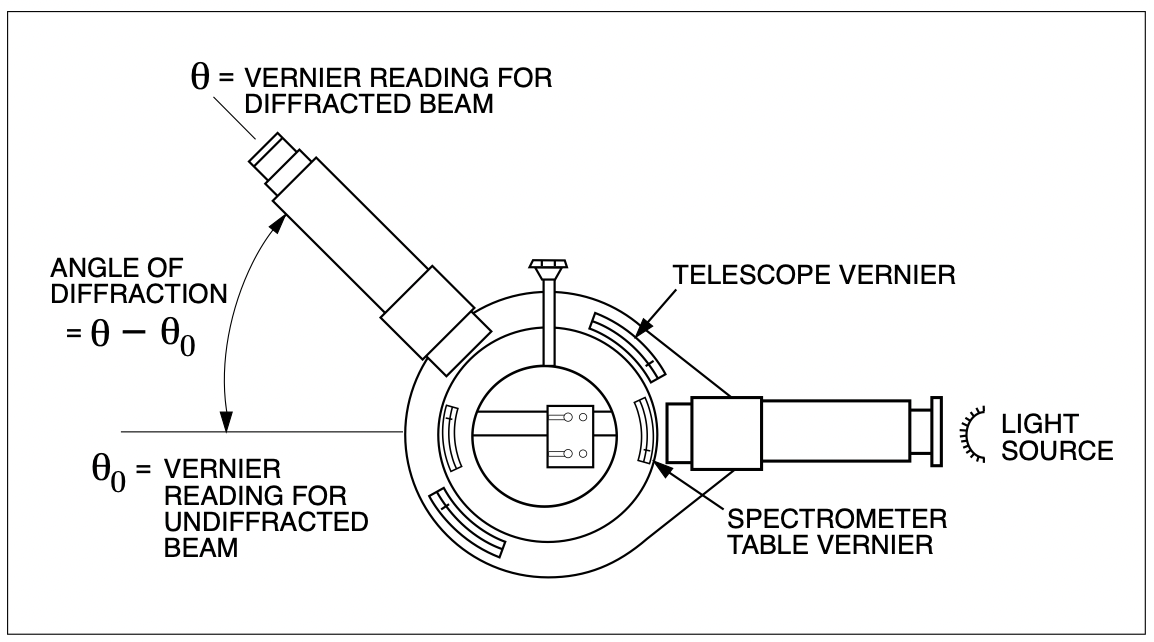
\includegraphics[scale=.5]{Immagini/spettrometro 1.png}
    \caption{Rappresentazione dell'apparato sperimentale}
    \label{Fig.1}
\end{figure}

Utilizzando come oggettro analizzatore un prisma a base triangolare, abbiamo studiato il fenomeno della dispersione, che si verifica quando la luce attraversa un mezzo dielettrico otticamente trasparente. Il fascio collimato, attraversando il prisma, nel nostro caso caratterizzato dalla presenza di due facce ottiche, viene scomposto in componenti di diverse lunghezze d'onda. Questo ci ha permesso di verificare la legge di Cauchy, che descrive il fenomeno della dispersione mettendo in relazione l'indice di rifrazione e la lunghezza d'onda attraverso la relazione:
\begin{equation}
n(\lambda)=A+\dfrac{B}{\lambda ^2}+\dfrac{C}{\lambda ^4} + ...
\end{equation}
La forma approssimata che si andrà a verificare è
$$
n(\lambda)=A+\dfrac{B}{\lambda ^2}
$$

Successivamente abbiamo lavorato con il reticolo, oggetto analizzatore composto da un insieme di fenditure equistanziate di uguale ampiezza. Esso ci ha permesso di studiare il fenomeno della diffrazione, poichè ci consente di osservare un'immagine costituita da massimi e minimi di intensità con posizioni angolari differenti. La legge riportata sotto è quella che abbiamo utilizzato e serve a descrivere il fenomeno nel caso di incidenza del raggio perpendicolare al reticolo:
\begin{equation}
    d\sin(\theta) = n\lambda
\label{rifrazione}
\end{equation}
Per quanto riguarda lo studio del gas ignoto abbiamo utilizzato due lampade ad arco, i due differenti mezzi analizzatori e le rispettive leggi.
